\chapter{Динамика Фридмана и уравнение состояния}

\lectureoverview{Однородное расширение необходимо отделять от локальной физики связанных систем, а внутреннюю геометрию — от формы вложения. Как только эти различия четко установлены, космологический принцип сводит метрику пространства-времени к одному масштабному фактору \(a(t)\) и одному параметру кривизны \(k\). Компонента время-время уравнения Эйнштейна тогда становится энергетическим уравнением Фридмана. Чтобы решить его, нам все еще нужно соотношение для вещества между давлением и плотностью энергии. Адиабатическая термодинамика и уравнение состояния \(P=w\rho\) дают \(\rho\propto a^{-3(1+w)}\), объединяя вещество, излучение и энергию вакуума в одной схеме.}

\section{Вопросы, уточняющие физическую картину}

\subsection{Может ли пространство периодически повторяться в пределах горизонта?}

Конечную плоскую Вселенную можно представить периодической ячейкой. Если бы эта ячейка была меньше наблюдаемой области, свет мог бы пересечь ее, и небо содержало бы повторяющиеся изображения одних и тех же структур. Обнаружить такие повторения труднее, чем просто узнать знакомую галактику: изображения приходят из разных направлений и эпох и изменены космической эволюцией. Тем не менее периодическая топология имеет наблюдательные следствия.

\begin{classroomqa}
\audiencequestion{Может ли вся Вселенная быть меньше наблюдаемой Вселенной?}
\lecturerresponse{Естественный вариант — периодически отождествленный тор. Тогда мы наблюдали бы повторяющиеся копии одной и той же физической области, образно говоря, видя самих себя через заднюю дверь. Поиски соответствующей космической периодичности не дали подтверждающих свидетельств, но действительно накладывают ограничения на малые фундаментальные ячейки. Такая возможность геометрически непротиворечива, но эти данные не говорят в пользу Вселенной, меньшей, чем уже наблюдаемая область. \lecturetimestamp{00:01:17--00:02:33}}
\end{classroomqa}

\subsection{Расширение не разрывает связанные системы}

Космическое расширение описывает крупномасштабное движение свободно движущегося вещества в усредненной космологической геометрии. Это не универсальное предписание, согласно которому всякая собственная длина должна увеличиваться. Электромагнитные силы связывают атомы, гравитация — планетные системы, а обычные молекулярные силы — твердые тела. Эти взаимодействия на таких масштабах неизмеримо сильнее космологической поправки.

\begin{classroomqa}
\audiencequestion{Вызывается ли расширение темной энергией, и почему атомы или планетные орбиты не расширяются вместе с пространством?}
\lecturerresponse{О том, что Вселенная расширяется, было известно еще до открытия темной энергии. Темная энергия изменяет расширение, ускоряя его; она не является ни определением расширения, ни его исходной причиной. Связанная система не следует хаббловскому потоку, поскольку в ней доминируют локальные силы. Ускоряющийся фон может вызвать чрезвычайно малое возмущение атома или орбиты, но обычное связывание восстанавливает почти неизменное равновесие, а не позволяет системе разлететься. \lecturetimestamp{00:02:36--00:06:50}}
\end{classroomqa}

\subsection{Энергия в зависящей от времени геометрии}

Оставшееся возражение касается не силы, а учета. Если связанная орбита непрерывно сопротивляется малому космологическому возмущению, откуда берется необходимая энергия? Эта посылка переносит закон сохранения из статического фона в пространство-время, у которого нет глобальной симметрии сдвига по времени.

\begin{classroomqa}
\audiencequestion{Откуда берется энергия, когда локальное связывание сопротивляется расширению?}
\lecturerresponse{Сохранение энергии в статическом мире следует из инвариантности относительно сдвига по времени: фон и его законы выглядят одинаково, если эксперимент сдвинуть по времени. Расширяющееся пространство-время не инвариантно относительно сдвига по времени в этом глобальном смысле, поэтому для всей Вселенной может не существовать единой сохраняющейся полной энергии. Локальное сохранение тензора энергии-импульса по-прежнему выполняется и ниже появится как уравнение непрерывности. Ложным оказывается наивное утверждение, будто глобально определенная космическая энергия должна оставаться постоянной, пока геометрия меняется. \lecturetimestamp{00:06:52--00:09:24}}
\end{classroomqa}

\subsection{Однородность — утверждение крупнозернистого описания}

Космологический принцип зависит от масштаба. Воздух в закрытой комнате может быть почти однородным в масштабе комнаты, но гранулярным на молекулярных масштабах. Вселенная точно так же содержит планеты, галактики, скопления и флуктуации плотности. Однородность и изотропия относятся к ее усредненному поведению на достаточно больших расстояниях, где эти структуры перестают выделять какое-либо место или направление.

\begin{classroomqa}
\audiencequestion{Противоречат ли связанные структуры малых масштабов однородности и изотропии?}
\lecturerresponse{Нет. Точная однородность нарушается на малых масштабах, как она нарушается и для воздуха, когда разрешаются отдельные молекулы. На масштабах в сотни миллионов световых лет и больше наблюдаемое распределение приблизительно однородно и не зависит от направления. За пределами области, которую мы можем наблюдать, однородность остается предположением, последствия которого нужно проверять, а не установленным фактом. \lecturetimestamp{00:09:27--00:10:55}}
\end{classroomqa}

\section{Однородность и изотропия как утверждения о метрике}

Однородность и изотропия — это геометрические утверждения прежде, чем они становятся динамическими. Уравнение Эйнштейна скажет нам, как геометрия меняется со временем. Сначала мы должны сказать, какой тип пространственной геометрии допустим в любой данный момент времени.

\begin{classroomqa}
\audiencequestion{Что математически означают однородность и изотропия?}
\lecturerresponse{Опишите пространство метрикой и выберите координаты \(x^i\) с началом в одной точке. Теперь выберите координаты \(y^i\) с началом в другой точке. Однородность означает, что преобразование может перенести начало координат, оставляя метрику в том же функциональном виде. Тогда каждая точка геометрически эквивалентна любой другой. Изотропия добавляет вращательную симметрию относительно каждой точки, так что ни одно направление не является предпочтительным. \lecturetimestamp{00:11:13--00:14:26}}
\end{classroomqa}

\begin{definition}
Пространство является \emph{однородным}, если изометрия может перевести любую точку в любую другую. Оно является \emph{изотропным} относительно точки, если повороты вокруг этой точки оставляют его геометрию неизменной. Пространство, которое однородно и изотропно, не имеет ни предпочтительного положения, ни предпочтительного направления.
\end{definition}

Евклидова плоскость делает определение наглядным. В декартовых координатах,
\begin{equation}
ds^2=dx_1^2+dx_2^2.
\label{eq:c04-flat-metric}
\end{equation}
Сдвинем начало координат на постоянные \(a_1\) и \(a_2\):
\begin{equation}
y_1=x_1+a_1,
\qquad
y_2=x_2+a_2.
\label{eq:c04-flat-translation}
\end{equation}
Поскольку \(dy_i=dx_i\), метрика в новых координатах имеет вид
\begin{equation}
ds^2=dy_1^2+dy_2^2.
\end{equation}
Символы, которыми обозначена точка, изменились, но правило расстояния — нет. Это простейшая реализация однородности. Повороты точно так же сохраняют метрику, так что плоскость также изотропна.

Сфера менее тривиальна лишь потому, что ее координаты менее удобны. Если выбрать южный полюс за начало, единичную двумерную сферу можно записать как
\begin{equation}
d\Omega_2^2=dr^2+\sin^2 r\,d\theta^2.
\label{eq:c04-sphere-metric}
\end{equation}
Повернем сферу так, чтобы восточный полюс стал новым началом. Координатное преобразование громоздко, но результатом снова будет уравнение~\eqref{eq:c04-sphere-metric}. Ни одна точка на круглой сфере геометрически не выделена.

\begin{classroomqa}
\audiencequestion{Является ли периодически отождествленный плоский тор одновременно однородным и изотропным?}
\lecturerresponse{Он однороден относительно трансляций: каждая точка в периодической ячейке имеет одну и ту же локальную геометрию. Полностью изотропным он не является, потому что отождествления выделяют предпочтительные периодические направления и длины. Взгляд вдоль одной из этих осей глобально отличается от взгляда в произвольном наклонном направлении. Поэтому тор дает наглядный пример однородности без полной изотропии. \lecturetimestamp{00:20:18--00:21:30}}
\end{classroomqa}

Наблюдаемая крупномасштабная однородность мотивирует космологический принцип внутри нашего горизонта. Распространение его на область за пределами наблюдаемой части — постулат, а не прямое наблюдение. Мы принимаем этот постулат, потому что он задает четко определенную геометрию, следствия которой можно сопоставить с данными.

\section{Внутренняя геометрия и вложение}

Когда пространство называют сферическим, возникает соблазн представить себе резиновую поверхность воздушного шара, помещенную в большую комнату. Эта картинка может помочь нам рисовать, но окружающая комната не является частью космологического утверждения. Важна \emph{внутренняя} геометрия: она состоит из расстояний и углов, измеримых наблюдателями, которые остаются внутри пространства.

\subsection{Замкнутые одномерные миры}

Рассмотрим замкнутый одномерный мир. Мы можем изобразить его окружностью, квадратом со скругленными углами или петлей в форме арахиса. Обитатель, ограниченный этой линией, измеряет только расстояние вдоль нее. Если две петли имеют одну и ту же полную длину, то их обитатели обнаружат одну и ту же внутреннюю геометрию, даже если рисунки выглядят совершенно по-разному.

\begin{figure}[htbp]
\centering
\includegraphics[width=0.72\textwidth]{lecture_04_figure_05.png}
\caption{Круглые и деформированные замкнутые петли, используемые для различения внутренней геометрии и формы вложения. Этот более поздний кадр сохраняет рисунки, сделанные в ходе более раннего обсуждения; существенное содержание приходится на 00:23:21--00:25:59.}
\label{fig:c04-intrinsic-board}
\lectureframe{00:59:54.899}
\end{figure}

Любая одномерная метрика локально плоская. Короткий участок нити можно выпрямить, не растягивая его, поэтому видимый изгиб в окружающей плоскости является внешней, а не внутренней кривизной. У замкнутой петли есть глобальный параметр — длина её контура, — но у неё нет внутреннего локального изгиба, который могли бы измерить её одномерные обитатели.

\begin{figure}[htbp]
\centering
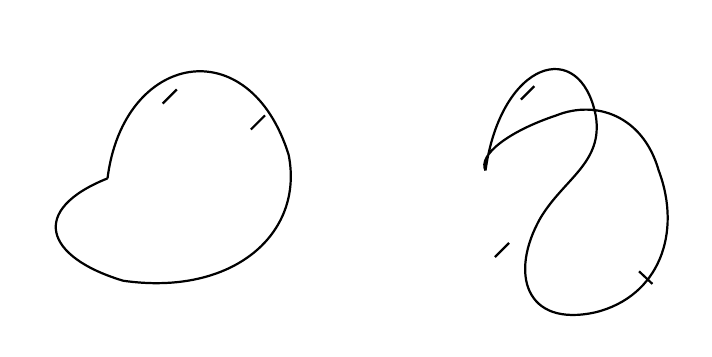
\begin{tikzpicture}[scale=1.0]
\draw[line width=0.8pt] (0,0)
  .. controls (0.2,1.6) and (1.8,1.9) .. (2.3,0.3)
  .. controls (2.5,-0.7) and (1.6,-1.5) .. (0.2,-1.3)
  .. controls (-0.8,-1.0) and (-1.0,-0.4) .. (0,0);
\draw[line width=0.8pt] (0.70,0.95) -- (0.88,1.13);
\draw[line width=0.8pt] (1.82,0.62) -- (2.00,0.80);

\draw[line width=0.8pt] (4.8,0.1)
  .. controls (5.0,1.5) and (6.0,1.8) .. (6.2,0.8)
  .. controls (6.3,0.2) and (5.8,0.0) .. (5.5,-0.5)
  .. controls (5.1,-1.2) and (5.3,-1.9) .. (6.2,-1.7)
  .. controls (7.0,-1.5) and (7.3,-0.7) .. (7.0,0.1)
  .. controls (6.8,0.8) and (6.2,1.0) .. (5.7,0.8)
  .. controls (5.1,0.6) and (4.7,0.3) .. (4.8,0.1);
\draw[line width=0.8pt] (5.25,1.00) -- (5.42,1.17);
\draw[line width=0.8pt] (5.10,-0.82) -- (4.92,-1.00);
\draw[line width=0.8pt] (6.75,-1.18) -- (6.92,-1.34);
\end{tikzpicture}
\caption{Аккуратное воспроизведение окружности и деформированной петли. Одинаковая длина контура означает одинаковую внутреннюю одномерную геометрию.}
\label{fig:c04-intrinsic-redraw}
\end{figure}

\begin{classroomqa}
\audiencequestion{Является ли конечный отрезок тем же типом одномерного пространства?}
\lecturerresponse{Нет. У отрезка есть две конечные точки, а у замкнутой петли — ни одной. Это топологическое различие является внутренним и не может быть устранено изгибанием любого из этих объектов в пространстве большей размерности. При фиксированной топологии отрезок характеризуется своей длиной, а замкнутая петля — длиной контура. \lecturetimestamp{00:26:00--00:26:39}}
\end{classroomqa}

\subsection{Почему вложения полезны, но необязательны}

Мы визуализируем одномерную окружность, помещая её в двумерное пространство, а двумерную сферу — в трёхмерное. Эта закономерность побуждает нас требовать четвёртого евклидова измерения, прежде чем обсуждать трёхсферу. Однако такое требование отражает особенности человеческой визуализации, а не математическую необходимость. Наш зрительный аппарат эволюционировал для ориентации в трёх измерениях; координаты и метрики позволяют нам рассуждать за пределами этого ограничения, не вводя буквальную внешнюю точку наблюдения.

\begin{classroomqa}
\audiencequestion{Могут ли дополнительные пространственные измерения существовать, но быть слишком малы, чтобы их можно было увидеть?}
\lecturerresponse{Да. Геометрия не требует, чтобы все измерения имели одну и ту же наблюдаемую протяжённость. Компактное измерение могло бы быть намного меньше масштабов, доступных обычному опыту. Однако суть здесь проще: независимо от того, существуют ли дополнительные измерения физически, размерность пространства вложения не требуется для определения внутренней метрики нашего трёхмерного пространства. \lecturetimestamp{00:29:55--00:30:12}}
\end{classroomqa}

\begin{classroomqa}
\audiencequestion{Как обитатель, ограниченный искривлённой линией, мог бы узнать, изогнута ли она?}
\lecturerresponse{Он не мог бы узнать этого, опираясь только на внутренние измерения. Представьте, что свет и материя ограничены оптическим волокном. Изгиб волокна без его растяжения изменяет вложение, но не расстояния и не времена прохождения сигналов, измеряемые вдоль него. Только сигнал, вышедший в окружающее пространство, мог бы выявить внешний изгиб. \lecturetimestamp{00:30:15--00:31:14}}
\end{classroomqa}

Этот мысленный эксперимент можно превратить в операциональную процедуру. Существо, ограниченное волокном, могло бы послать сигнал, например достаточно энергичный фотон, и обнаружить внешнее направление только в том случае, если бы сигнал покинул волокно, а затем вернулся по пути, недоступному в рамках одномерной метрики. В том же духе утверждение о том, что обычное пространство имеет три больших измерения, в конечном счёте является экспериментальным, а не выводом из того, что человеческий разум способен наглядно представить.

\begin{classroomqa}
\audiencequestion{Если всякое одномерное пространство локально плоское, то должно ли всякое двумерное пространство тоже быть локально плоским?}
\lecturerresponse{Нет. Лист, свернутый в цилиндр, остается внутренне плоским: его можно развернуть без растяжения. Полусферу нельзя распрямить на плоскость без растяжения или разрыва, поэтому она обладает внутренней кривизной. Всякий достаточно малый участок выглядит приблизительно евклидовым, но на конечном масштабе появляются измеримые отклонения. Различие между цилиндром и сферой — это в точности различие между внешним изгибом и внутренней кривизной. \lecturetimestamp{00:31:14--00:35:00}}
\end{classroomqa}

\begin{classroomqa}
\audiencequestion{Означает ли внутренняя кривизна обязательно, что присутствует гравитационное поле?}
\lecturerresponse{В общей теории относительности кривизна пространства-времени является инвариантным проявлением приливной гравитации. Поэтому космологическая пространственная кривизна \(k/a^2\) есть часть гравитационной геометрии, а не просто изгиб в воображаемом внешнем пространстве. Вещество влияет на кривизну через уравнение Эйнштейна, но не следует заострять это утверждение до «кривизна существует только там, где находится вещество»: вакуумное пространство-время может нести вейлевскую кривизну, как вне звезды или в гравитационной волне. \lecturetimestamp{00:35:01--00:35:51}}
\end{classroomqa}

Теперь введем крупномасштабную идеализацию. Усредним по звездам, галактикам, скоплениям и локальным неоднородностям, подобно тому как, описывая Землю как круглую, пренебрегают горами. Получающуюся пространственную геометрию будем считать однородной и изотропной. При этих предположениях возможны три варианта геометрии постоянной кривизны: плоская, сферическая и гиперболическая.

\section{Анзац Фридмана—Робертсона—Уокера и три случая кривизны}

Предположения о симметрии сводят геометрию к одному масштабу, зависящему от времени, и одному дискретному знаку кривизны. В сопутствующих координатах анзац Фридмана—Робертсона—Уокера имеет вид
\begin{equation}
ds^2=-dt^2+a(t)^2\,d\Sigma_k^2,
\qquad
k\in\{-1,0,+1\}.
\label{eq:c04-frw}
\end{equation}
Временная координата — это собственное время сопутствующих наблюдателей. Однородность допускает зависимость \(a\) от времени, но не от положения, тогда как изотропия запрещает выделенное пространственное направление.

\begin{figure}[htbp]
\centering
\includegraphics[width=0.74\textwidth]{lecture_04_figure_02.png}
\caption{Три пространственные метрики постоянной кривизны, сгруппированные под общим масштабным множителем. Кадр был снят позже, после того как на доске накопился другой материал, но он сохраняет обсуждение метрик из 00:40:23--00:42:42.}
\label{fig:c04-frw-board}
\lectureframe{00:45:48.386}
\end{figure}

Используя радиальную координату \(r\) и метрику единичной двумерной сферы \(d\Omega_2^2\), получаем три нормированные пространственные метрики
\begin{align}
d\Sigma_0^2 &= dr^2+r^2d\Omega_2^2,
&& k=0,
\label{eq:c04-flat-space}\\
d\Sigma_{+1}^2 &= dr^2+\sin^2 r\,d\Omega_2^2,
&& k=+1,
\label{eq:c04-spherical-space}\\
d\Sigma_{-1}^2 &= dr^2+\sinh^2 r\,d\Omega_2^2,
&& k=-1.
\label{eq:c04-hyperbolic-space}
\end{align}
Следовательно, в фиксированный момент времени пространство является плоским, положительно искривленным или отрицательно искривленным. Умножение на \(a(t)^2\) изменяет все пространственные расстояния в одном и том же отношении, сохраняя нормированную форму.

Рассмотрим две галактики с фиксированным сопутствующим расстоянием \(\Delta\chi\). Их физическое расстояние равно
\begin{equation}
D(t)=a(t)\Delta\chi.
\end{equation}
Дифференцируя и исключая \(\Delta\chi\), получаем
\begin{equation}
\dot D=\dot a\,\Delta\chi
      =\frac{\dot a}{a}D
      =H(t)D,
\qquad
H(t)\equiv\frac{\dot a}{a}.
\label{eq:c04-hubble-law}
\end{equation}
Тем самым закон Хаббла кинематически следует из однородного масштабирования. Параметр Хаббла может меняться со временем, но в любой фиксированный космический момент он везде одинаков.

\section{От уравнения Эйнштейна к уравнению Фридмана}

Метрика говорит нам, как измеряются расстояния, но не то, как эволюционирует \(a(t)\). Для искривленного пространства-времени требуется уравнение Эйнштейна. Вычисление каждого символа Кристоффеля и каждой компоненты кривизны только затемнило бы физический ход рассуждения, поэтому мы воспользуемся формой, диктуемой симметрией, и выделим ее время-время-компоненту.

В единицах, где \(c=1\), и при временно опущенной космологической постоянной полное тензорное уравнение имеет вид
\begin{equation}
G_{\mu\nu}
\equiv
R_{\mu\nu}-\frac12 g_{\mu\nu}R
=8\pi G\,T_{\mu\nu}.
\label{eq:c04-einstein}
\end{equation}
Слева стоит геометрия; справа — плотность энергии, плотность импульса, давление и напряжения. Множитель \(1/3\) не входит в полное тензорное уравнение. Он появляется только после того, как компонента время–время приведена к форме Фридмана.

\begin{figure}[htbp]
\centering
\includegraphics[width=0.78\textwidth]{lecture_04_figure_03.png}
\caption{Промежуточное состояние записи уравнения Эйнштейна на доске. Видна геометрическая левая часть, тогда как тензор материи еще неразборчив, а показанная нормировка неполна. В уравнении~\eqref{eq:c04-einstein} записано стандартное полное тензорное уравнение, используемое в выводе.}
\label{fig:c04-einstein-board}
\lectureframe{00:48:19.394}
\end{figure}

Для однородной жидкости, покоящейся в сопутствующих координатах,
\begin{equation}
T_{00}=\rho.
\label{eq:c04-energy-density}
\end{equation}
У компоненты время–время тензора Эйнштейна есть полезное структурное свойство. Вторые производные в ней сокращаются, оставляя один член, квадратичный по первой производной по времени, и один член, обусловленный пространственной кривизной:
\begin{equation}
G_{00}=3\left[
\left(\frac{\dot a}{a}\right)^2+\frac{k}{a^2}
\right].
\label{eq:c04-g00}
\end{equation}
Подстановка уравнений~\eqref{eq:c04-energy-density} и \eqref{eq:c04-g00} в уравнение~\eqref{eq:c04-einstein} дает первое уравнение Фридмана,
\begin{equation}
\boxed{
\left(\frac{\dot a}{a}\right)^2+\frac{k}{a^2}
=\frac{8\pi G}{3}\rho
}.
\label{eq:c04-friedmann}
\end{equation}
Эквивалентно,
\begin{equation}
H^2=\frac{8\pi G}{3}\rho-\frac{k}{a^2}.
\label{eq:c04-friedmann-energy}
\end{equation}
Уравнение~\eqref{eq:c04-friedmann-energy} имеет в точности тот вид, который был получен в предыдущем ньютоновском рассуждении. Там постоянная интегрирования интерпретировалась как полная механическая энергия или условие убегания для сферы вещества. Общая теория относительности ставит собственную пространственную кривизну на то же математическое место. Это совпадение не случайно: в достаточно малой области эффектами кривизны можно пренебречь, и релятивистская космология должна воспроизводить локальное ньютоновское поведение. Теория относительности также проясняет, что \(\rho\) означает полную плотность энергии, так что релятивистские частицы и фотоны гравитируют, хотя нерелятивистский аргумент, основанный на плотности массы, их бы упустил.

\begin{classroomqa}
\audiencequestion{Почему в метрике нет членов, смешивающих пространство и время?}
\lecturerresponse{Смешанный член вел бы себя как выделенный пространственный вектор или поток относительно сопутствующих наблюдателей. Точная однородность и изотропия не оставляют никакого такого направления. Поэтому в координатах, приспособленных к космическому веществу, вектор сдвига обращается в нуль, и метрика принимает блочно-диагональный вид из уравнения~\eqref{eq:c04-frw}. Если предполагаемые симметрии сохраняются, это не дополнительное динамическое предположение, а их геометрическое следствие. \lecturetimestamp{00:58:27--00:59:08}}
\end{classroomqa}

\begin{classroomqa}
\audiencequestion{Почему достаточно компоненты времени-времени, и куда делись вторые производные?}
\lecturerresponse{Однородный и изотропный анзац содержит только одну неизвестную функцию, \(a(t)\). Смешанные компоненты сводятся к тождествам, тогда как пространственные компоненты связаны с уравнением для компоненты времени-времени и законом сохранения энергии-импульса. Их можно объединить в уравнение ускорения, содержащее \(\ddot a\), однако компонента тензора Эйнштейна времени-времени особенна: члены со вторыми производными в ней сокращаются, оставляя уравнение энергии первого порядка~\eqref{eq:c04-friedmann}. Одного нетривиального уравнения вместе с законом эволюции содержимого достаточно, чтобы определить единственную геометрическую степень свободы. \lecturetimestamp{00:59:09--01:00:56}}
\end{classroomqa}

\section{Как разрежается содержимое Вселенной}

Уравнение Фридмана не замкнуто, пока \(\rho\) не известна как функция \(a\). Геометрия даёт одно уравнение; содержимое Вселенной должно дать второе соотношение.

Для нерелятивистской материи число частиц в сопутствующем объёме фиксировано, тогда как физический объём растёт как \(a^3\). Пренебрегая малыми кинетическими энергиями частиц,
\begin{equation}
\rho_{\mathrm m}(a)=\frac{\rho_{\mathrm m,0}}{a^3}.
\label{eq:c04-matter-scaling}
\end{equation}
Здесь нормировку \(a=1\) можно выбрать на любой удобной опорной эпохе; непосредственный смысл имеют только отношения значений масштабного фактора.

\begin{classroomqa}
\audiencequestion{Если плоская Вселенная бесконечна, что означает уменьшение \(a\) по мере приближения к Большому взрыву?}
\lecturerresponse{Бесконечное плоское пространство остаётся бесконечным при любом ненулевом значении \(a\); все конечные сопутствующие расстояния умножаются на один и тот же убывающий множитель. Абсолютная нормировка \(a\) в плоском случае произвольна, так что инвариантный смысл имеет только \(a(t_2)/a(t_1)\). Для замкнутой сферической Вселенной \(a\) естественно является её радиусом кривизны, а для гиперболической Вселенной задаёт радиус кривизны. Предел \(a\to0\) указывает на космологическую сингулярность, а не на обычный конечный шар, находящийся во внешнем пространстве. \lecturetimestamp{01:05:06--01:05:53}}
\end{classroomqa}

Излучение теряет энергию двумя способами. Его числовая плотность убывает обратно пропорционально объёму, а длина волны каждого фотона растягивается пропорционально \(a\), уменьшая его энергию ещё на множитель \(a^{-1}\). Поэтому
\begin{equation}
\rho_{\mathrm r}(a)=\frac{\rho_{\mathrm r,0}}{a^4}.
\label{eq:c04-radiation-scaling}
\end{equation}
Поскольку \(a^{-4}\) при переходе к прошлому растёт быстрее, чем \(a^{-3}\), излучение начинает доминировать достаточно рано, даже если гораздо позже доминирует материя.

Если бы единственными компонентами были материя и излучение, знак \(k\) в значительной степени определял бы будущее: \(k=+1\) допускает повторное сжатие, \(k=0\) — предельный случай, который расширяется вечно, замедляясь, а \(k=-1\) расширяется вечно, причём кривизна в конце концов становится существенной. Тёмная энергия разрушает эту простую связь. Замкнутая Вселенная может расширяться вечно, и сама по себе пространственная плоскостность не определяет конечную судьбу.

\section{Уравнение состояния и закон непрерывности}

Вместо того чтобы запоминать отдельный закон разрежения для каждой компоненты, будем характеризовать её уравнением состояния. Эта программа состоит из двух частей. Сначала выведите \(\rho(a)\) для заданной связи между давлением и плотностью энергии. Затем определите эту связь из микроскопической физики вещества, излучения или вакуума. Для этой лекции достаточно первой части.

Давление — это поток импульса. Молекулы, ударяясь о стенку ящика, меняют свой импульс на противоположный и давят на стенку; более быстрые частицы передают больший импульс и создают большее давление. Поэтому после задания типа среды плотность энергии и давление уже нельзя выбирать независимо. Для простой космологической компоненты пишем
\begin{equation}
P=w\rho,
\label{eq:c04-equation-state}
\end{equation}
где \(w\) безразмерна в единицах \(c=1\). У холодной материи давление пренебрежимо мало, и потому \(w=0\). Для излучения \(w=1/3\), причём множитель \(1/3\) отражает усреднение по трём пространственным направлениям.

\begin{figure}[htbp]
\centering
\includegraphics[width=0.82\textwidth]{lecture_04_figure_06.png}
\caption{На доске собраны законы масштабирования материи и излучения, а уравнение состояния записано как \(P=W\rho\). Мы используем общепринятое строчное \(w\).}
\label{fig:c04-equation-state-board}
\lectureframe{01:15:08.166}
\end{figure}

\subsection{Термодинамика в сопутствующем ящике}

Рассмотрим сопутствующий ящик с физическим объёмом \(V\), плотностью энергии \(\rho\) и полной энергией
\begin{equation}
E=\rho V.
\end{equation}
Первый закон имеет вид
\begin{equation}
dE=T\,dS-P\,dV.
\end{equation}
Космологическое расширение рассматривается как адиабатическое, так что для сопутствующего ящика \(dS=0\) и
\begin{equation}
dE=-P\,dV.
\label{eq:c04-adiabatic-first-law}
\end{equation}
Знак минус означает, что расширяющаяся система совершает работу и теряет внутреннюю энергию. Независимое дифференцирование \(E=\rho V\) даёт
\begin{equation}
dE=\rho\,dV+V\,d\rho.
\end{equation}
Приравнивая эти два выражения, получаем
\begin{align}
\rho\,dV+V\,d\rho&=-P\,dV,\\
V\,d\rho&=-(\rho+P)\,dV.
\label{eq:c04-volume-continuity}
\end{align}
С учётом \(P=w\rho\)
\begin{equation}
\frac{d\rho}{\rho}=-(1+w)\frac{dV}{V}.
\end{equation}
Интегрирование даёт
\begin{equation}
\rho\propto V^{-(1+w)}.
\end{equation}
Поскольку сопутствующий объём масштабируется как \(V\propto a^3\),
\begin{equation}
\boxed{\rho(a)\propto a^{-3(1+w)}}.
\label{eq:c04-density-scaling}
\end{equation}
В дифференциальной форме то же утверждение есть локальное уравнение сохранения энергии
\begin{equation}
\dot\rho+3H(\rho+P)=0.
\label{eq:c04-continuity}
\end{equation}
Этот локальный закон сохранения остаётся точным, хотя изменяющаяся космологическая геометрия и не обязана допускать глобально сохраняющуюся полную энергию.

Отсюда сразу следуют два знакомых случая:
\begin{align}
w=0
&\quad\Longrightarrow\quad
\rho_{\mathrm m}\propto a^{-3},\\
w=\frac13
&\quad\Longrightarrow\quad
\rho_{\mathrm r}\propto a^{-4}.
\end{align}
Дополнительная обратная степень у излучения — это термодинамическое выражение космологического красного смещения.

\begin{classroomqa}
\audiencequestion{Какое излучение остаётся сегодня во Вселенной?}
\lecturerresponse{В аудитории прежде всего указывают на космический микроволновый фон, реликтовую фотонную ванну из горячей ранней Вселенной. Сейчас излучение составляет малую долю полной космической плотности энергии, но его масштабирование как \(a^{-4}\) означает, что, если проследить уравнения достаточно далеко назад, оно обгоняет материю. Точные современные доли задаются наблюдениями и для этого аргумента о масштабировании не нужны. \lecturetimestamp{01:26:53--01:28:34}}
\end{classroomqa}

\section{Энергия вакуума и несостоятельность правила «кривизна — судьба»}

Для тёмной энергии вводится уравнение состояния
\begin{equation}
P=-\rho,
\qquad
w=-1.
\label{eq:c04-vacuum-eos}
\end{equation}
Отрицательное давление — это натяжение: вместо того чтобы толкать стенку ящика наружу, содержимое тянет её внутрь. Растянутая пружина — знакомый объект с натяжением, хотя это лишь аналогия, а не микроскопическая модель энергии вакуума.

\begin{classroomqa}
\audiencequestion{Связано ли отрицательное давление с абсолютным нулём?}
\lecturerresponse{В каком-либо простом общем смысле — нет. Охлаждение обычного вещества до нулевой температуры само по себе не приводит к космологическому уравнению состояния \(P=-\rho\). Этот обмен репликами полезен тем, что различает тепловое давление и напряжение вакуума: энергия вакуума характеризуется лоренц-инвариантным тензором энергии-импульса, пространственные компоненты которого действуют как отрицательное давление. Её микроскопическое происхождение — отдельный вопрос. \lecturetimestamp{01:31:01--01:31:46}}
\end{classroomqa}

Подстановка \(w=-1\) в уравнение~\eqref{eq:c04-density-scaling} даёт
\begin{equation}
\rho_\Lambda\propto a^0=\text{constant}.
\label{eq:c04-vacuum-density}
\end{equation}
По мере расширения сопутствующей области её объём и полная энергия вакуума растут вместе, так что энергия на единицу объёма остаётся неизменной. Член работы в уравнении~\eqref{eq:c04-adiabatic-first-law} объясняет такое поведение, потому что \(P\) отрицательно. Если присутствует такая компонента, положительная пространственная кривизна уже не гарантирует повторного сжатия.

\begin{classroomqa}
\audiencequestion{Куда в этой картине входят тёмная материя, чёрные дыры и другие компактные объекты?}
\lecturerresponse{На масштабах, больших по сравнению с расстояниями между ними, любая нерелятивистская компонента, случайные скорости которой малы, входит в плотность бездавленной материи. Это включает обычное вещество, холодную тёмную материю и популяцию компактных объектов, таких как чёрные дыры. Их локальная структура сложна, но после усреднения их среднее космологическое уравнение состояния приблизительно равно \(w=0\). \lecturetimestamp{01:33:34--01:34:10}}
\end{classroomqa}

\begin{classroomqa}
\audiencequestion{Воспроизводят ли релятивистские уравнения найденные ранее решения с доминированием материи и излучения?}
\lecturerresponse{Да. При \(k=0\) подстановка \(\rho_{\mathrm m}\propto a^{-3}\) в уравнение Фридмана даёт \(\dot a^2\propto a^{-1}\) и, следовательно, \(a(t)\propto t^{2/3}\). Подстановка \(\rho_{\mathrm r}\propto a^{-4}\) даёт \(\dot a^2\propto a^{-2}\) и \(a(t)\propto t^{1/2}\). Общая теория относительности меняет интерпретацию и расширяет набор возможных источников, но сохраняет эти решения. \lecturetimestamp{01:34:14--01:35:12}}
\end{classroomqa}

\begin{classroomqa}
\audiencequestion{На какую силу была бы похожа тёмная энергия в ньютоновской картине?}
\lecturerresponse{Положительная космологическая постоянная создаёт отталкивающее относительное ускорение, пропорциональное расстоянию,
\[
\ddot D=\frac{\Lambda}{3}D
\]
в единицах \(c=1\). Отрицательная космологическая постоянная меняет знак на противоположный и действует притягивающе. Поскольку эффект положительной \(\Lambda\) растёт с расстоянием, он может в конце концов начать доминировать над материей и кривизной; тогда даже Вселенная с \(k=+1\) может продолжать расширяться. Эта ньютоновская форма — лишь полезная тень релятивистской динамики. \lecturetimestamp{01:35:13--01:36:55}}
\end{classroomqa}

\section{Что нам понадобится дальше}

Космологический принцип — это усреднённое геометрическое утверждение: после сглаживания локальной структуры каждая точка и каждое направление эквивалентны. Он ограничивает пространственную метрику тремя случаями постоянной кривизны и сводит всю временную зависимость к \(a(t)\):
\begin{equation}
ds^2=-dt^2+a(t)^2d\Sigma_k^2.
\end{equation}
Тогда сопутствующие расстояния подчиняются соотношению \(\dot D=HD\), тогда как связанные системы не обязаны следовать этому потоку.

Уравнение Эйнштейна для компоненты время-время придаёт анзацу динамику:
\begin{equation}
H^2+\frac{k}{a^2}=\frac{8\pi G}{3}\rho.
\end{equation}
Сходство с ньютоновским уравнением энергии не случайно, но в общей теории относительности место интеграционной постоянной занимает внутренняя кривизна пространства, и вклад может вносить любая форма энергии.

Оставшееся соотношение задаётся термодинамикой. Для адиабатически расширяющейся компоненты с \(P=w\rho\),
\begin{equation}
\dot\rho+3H(\rho+P)=0,
\qquad
\rho\propto a^{-3(1+w)}.
\end{equation}
Для вещества, излучения и энергии вакуума это даёт соответственно
\begin{equation}
w=0,\qquad w=\frac13,\qquad w=-1.
\end{equation}
Разные темпы их разрежения определяют, какая компонента управляет расширением в каждую эпоху. Следующая задача — понять физику, стоящую за этими уравнениями состояния и за ускорением, порождаемым энергией вакуума.
